\documentclass{beamer}
\usepackage[utf8]{inputenc}
\usepackage[
backend=biber,
style=authoryear,
citestyle=authoryear
]{biblatex}
\usepackage{caption}
\usepackage{subcaption}

\addbibresource{refs.bib}

\setbeamertemplate{navigation symbols}{}
\usetheme{Frankfurt}
\useinnertheme{circles}
\definecolor{blue}{rgb}{0,0.15,0.6}
\setbeamercolor{headline}{fg=blue}

\title{Measuring Rhetorical Similarity with Machine Learning}

\author{Nicolai Berk}
\institute{University of Amsterdam}

\date{July 9, 2020}

\begin{document}

\maketitle

\section{Introduction}

\begin{frame}{Relevance}
    Group similarity of interest for many areas in political science:
    \begin{itemize}
        \item Representation
        \begin{itemize}
            \item Do certain (e.g. female/working class/PoC) MPs communicate differently?
            \item How similar is legislation to interest group's demands?
            \item Do MP's become more similar over time?
            \item Are directly elected MPs communicating differently?
        \end{itemize}
        \item Government formation
        \begin{itemize}
            \item Which parties communicate more similar and are more likely to form a coalition?
        \end{itemize}
        \item Party Competition
        \begin{itemize}
            \item Did parties become more or less similar to each other?
            \item Did parties fill political opportunity spaces opened by other parties?
            \item Which MPs are likely to leave their party?
        \end{itemize}
        \item Polarisation, ...
    \end{itemize}
\end{frame}

\begin{frame}{Current Methods}
    \begin{itemize}
        \item Simple similarity measures: cosine, jaccard \newline
        $\rightarrow$ no weighting of terms
        \item Scaling methods: WORDSCORE, WORDFISH (\cite{Laver2003, Slapin2008}) \newline
        $\rightarrow$ no similarity measures, cannot measure similarity of a document to a collection of texts
        \item \cite{Peterson2018}: Machine learning accuracy to measure polarisation
        $\rightarrow$ no estimates for single texts
        \item[$\rightarrow$]\textbf{Use ML to scale texts on 'groupness'}
    \end{itemize}
\end{frame}

\section{Method}

\begin{frame}{A supervised ML measure of group similarity}
    \begin{enumerate}
        \item Pre-process texts
        \item Select well-performing classifier
        \item Balance data, using SMOTE (\cite{Chawla2002})
        \item BoW-classifier trained on full set
        \item Predicted probabilities assigned to all texts
        \item Train one classifier/time-period to 'control' for changing language
    \end{enumerate}
\end{frame}


\section{Validity}
\begin{frame}{Application}
\begin{itemize}
    \item How similar are speakers and parties to the radical right?
    \item Parliamentary speeches from lower Chambers in AT, DE, NL (\cite{Rauh2020})
    \item estimates of similarity to radical right party obtained using Python's \texttt{scikit-learn}
    \item Logistic regression on unstemmed text, tfidf-weighted
\end{itemize}
\end{frame}

\begin{frame}{Validation}
    Three approaches
    \begin{itemize}
        \item Content of RR language
        \item Government formations with RR participation (AT \& NL)
        \item Speaker estimates of party exits (DE \& NL)
    \end{itemize}
\end{frame}

\begin{frame}{Best predictor Words}
\begin{figure}
     \centering
     \begin{subfigure}[b]{0.25\textwidth}
         \centering
         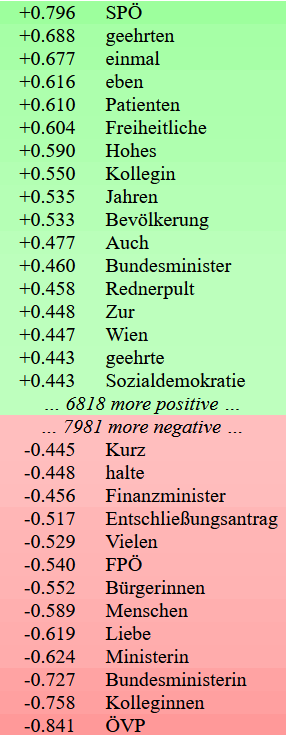
\includegraphics[width=\textwidth]{Presentation/bestPred_at.png}
         \caption{Austria}
     \end{subfigure}
     \hfill
     \begin{subfigure}[b]{0.235\textwidth}
         \centering
         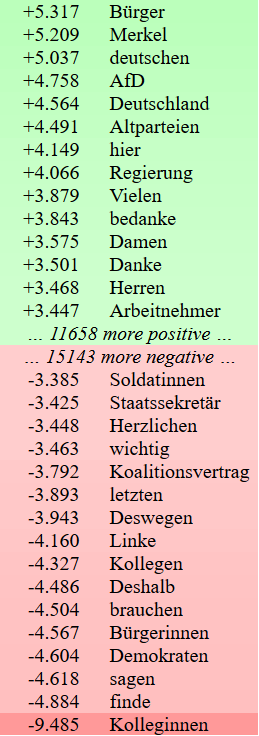
\includegraphics[width=\textwidth]{Presentation/bestPred_de.png}
         \caption{Germany}
     \end{subfigure}
     \hfill
     \begin{subfigure}[b]{0.235\textwidth}
         \centering
         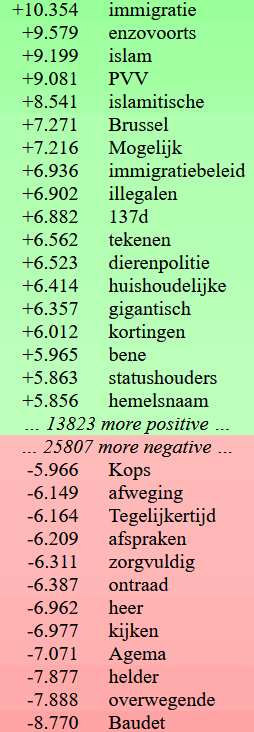
\includegraphics[width=\textwidth]{Presentation/bestPred_nl.png}
         \caption{Netherlands}
     \end{subfigure}
\end{figure}
\end{frame}


\begin{frame}[allowframebreaks]{Best predictor Words}
What distinguishes the radical right in \textbf{Austria}?
\begin{itemize}
    \item talking about \textbf{opposition}
    \item talking about Vienna (SD-governed)
    \item talking about health reform (RR-led ministry)
    \item less likely to address house as colleagues
    \item less likely to use gender-inclusive language
\end{itemize}

\framebreak
What distinguishes the radical right in \textbf{Germany}?
\begin{itemize}
    \item talking about \textbf{government}
    \item talking about Germany
    \item less likely to address house as colleagues
    \item less likely to use gender-inclusive language
    \item less causal language
\end{itemize}
\framebreak
What distinguishes the radical right in \textbf{the Netherlands}?
\begin{itemize}
    \item strong immigration focus
    \item more informal language
    \item less nuancing language
\end{itemize}

\end{frame}

\begin{frame}[allowframebreaks]{Radical-right government participation}
\begin{figure}
    \centering
    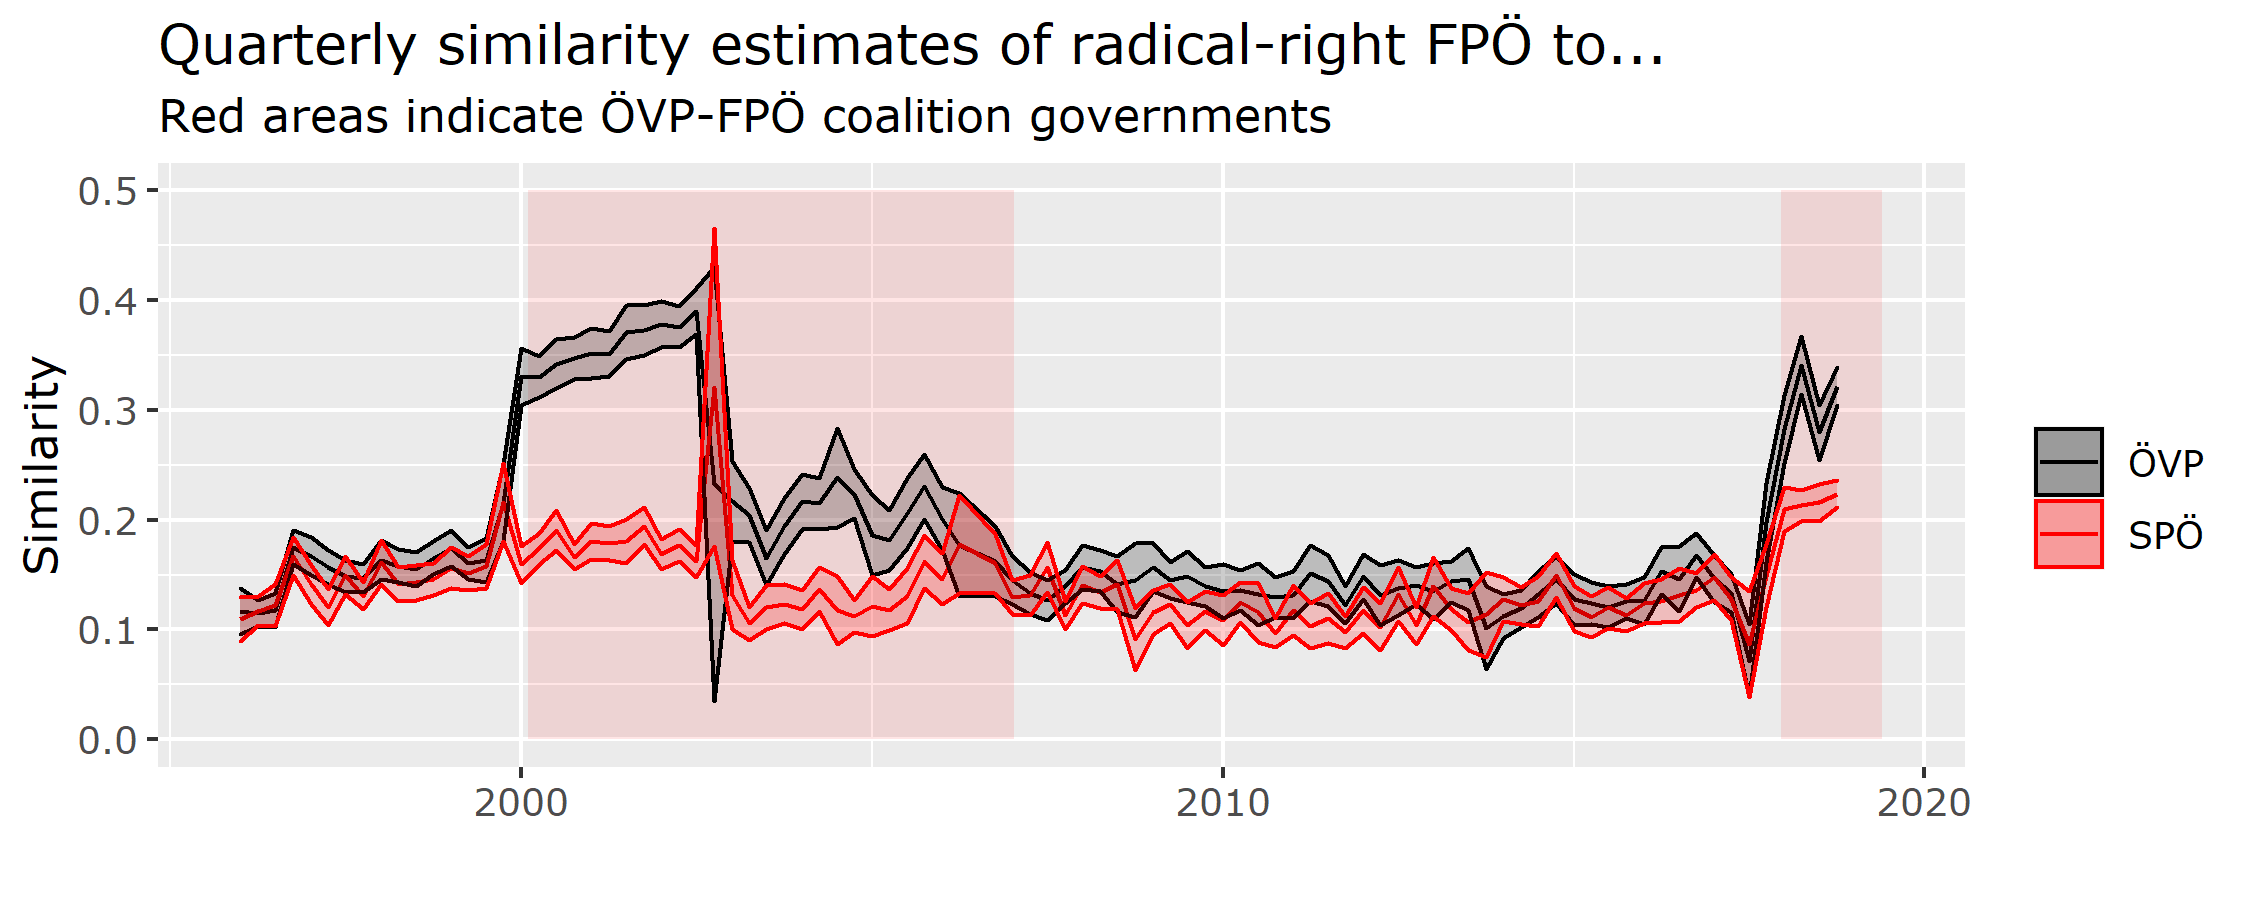
\includegraphics[width = \textwidth]{AT/vis/AT_fp_paper.png}
\end{figure}

\begin{figure}
        \centering
        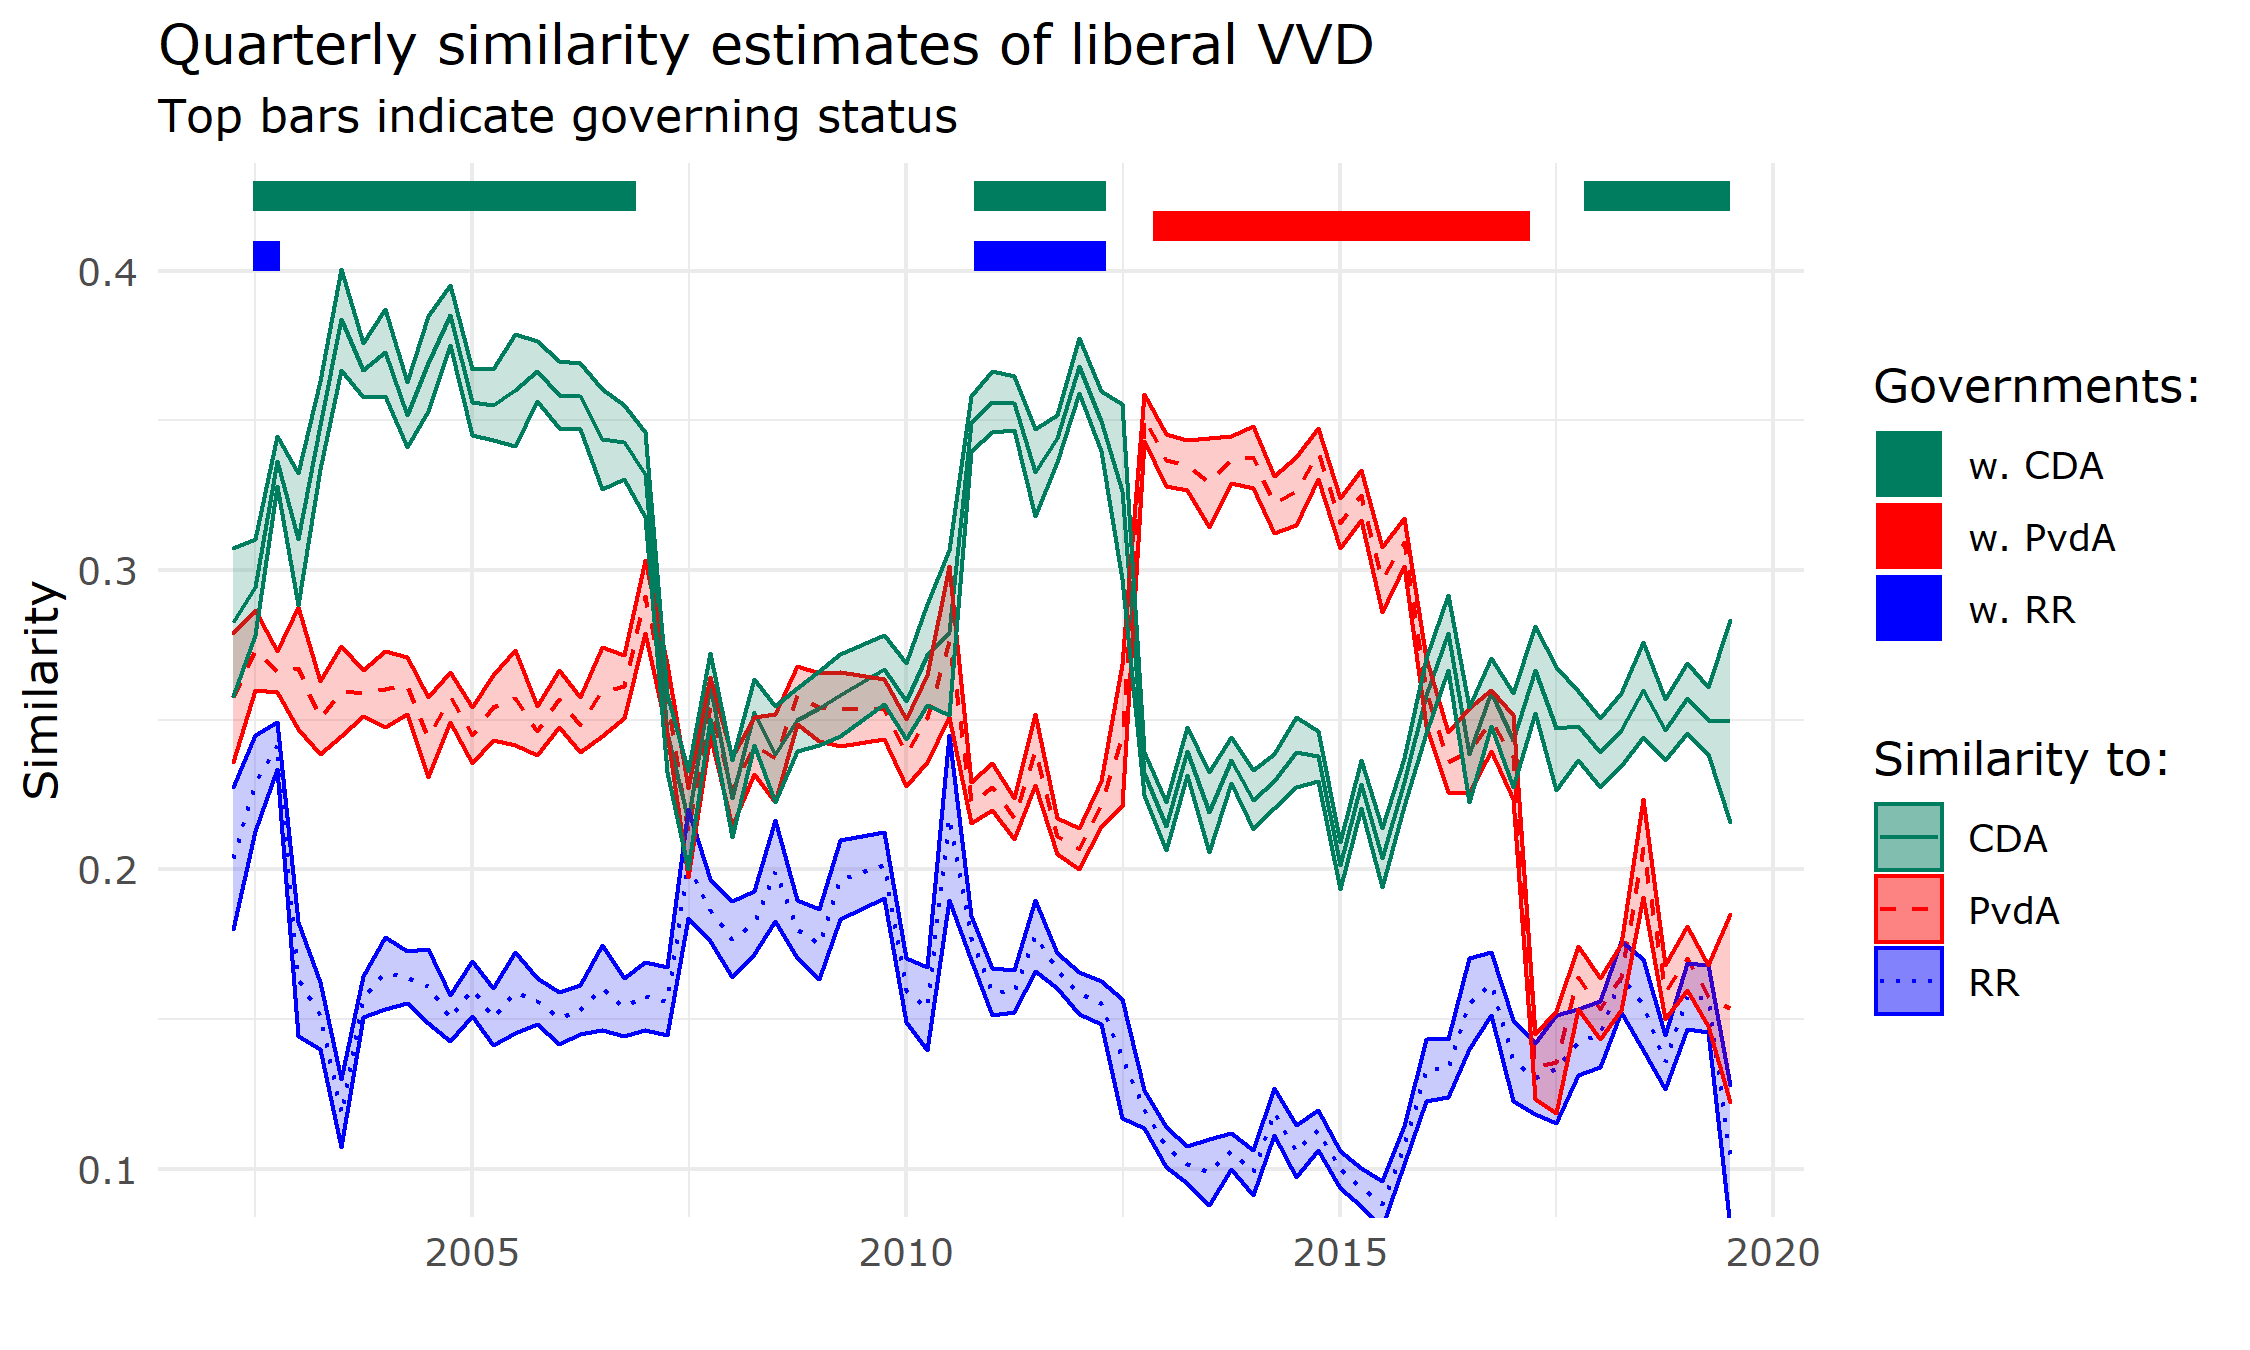
\includegraphics[width = \textwidth]{NL/vis/NL_vvd_sim.png}
\end{figure}
\end{frame}




\begin{frame}[allowframebreaks]{Speaker distribution}
    Leaving the AfD
    \begin{itemize}
        \item One day after the national election in 2017, Frauke Petry and Mario Mieruch left the party
        \item They became independent members of the Bundestag
    \end{itemize}\medskip

    Leaving the VVD
    \begin{itemize}
        \item Geert Wilders left the VVD in September 2004
        \item this followed a rift with his party over the immigration issue
        \item as well as a series of escalations (position paper in July, vote on Turkey end of August)
    \end{itemize}
    \framebreak
    \begin{figure}
        \centering
        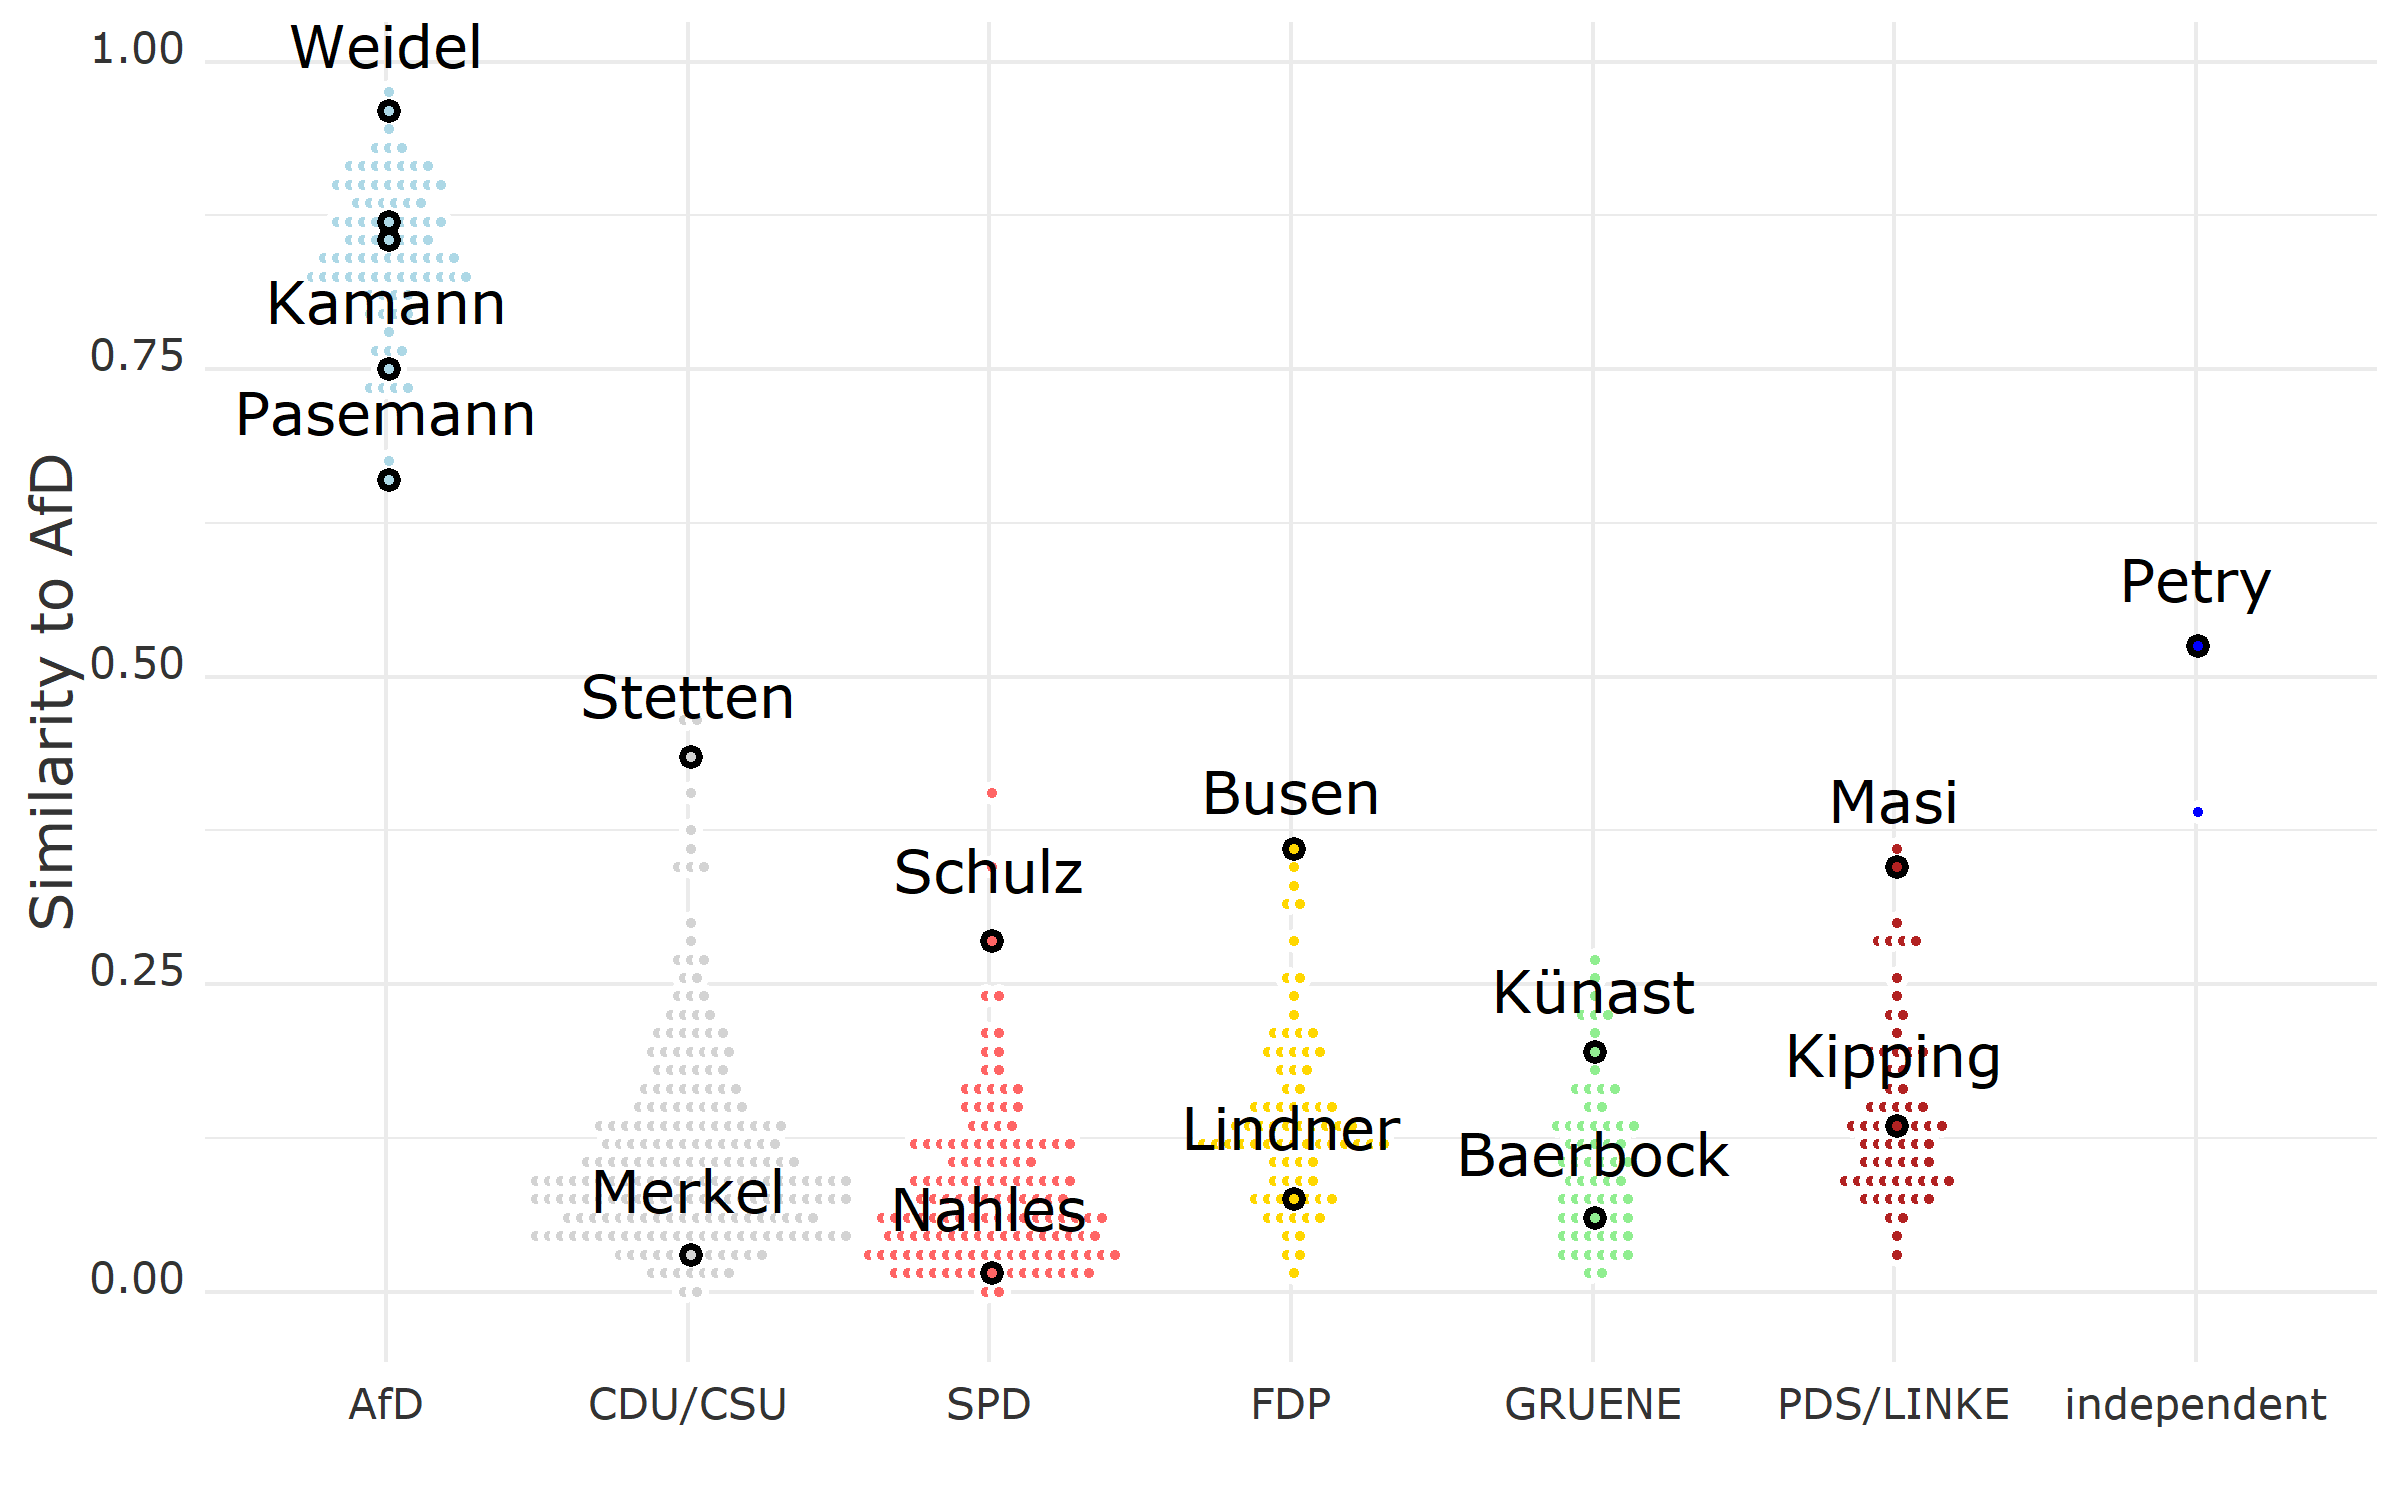
\includegraphics[width = \textwidth]{DE/vis/DE_speakers_PA.png}
        \caption{Speakers in the current German Bundestag.}
    \end{figure}
    \begin{figure}
        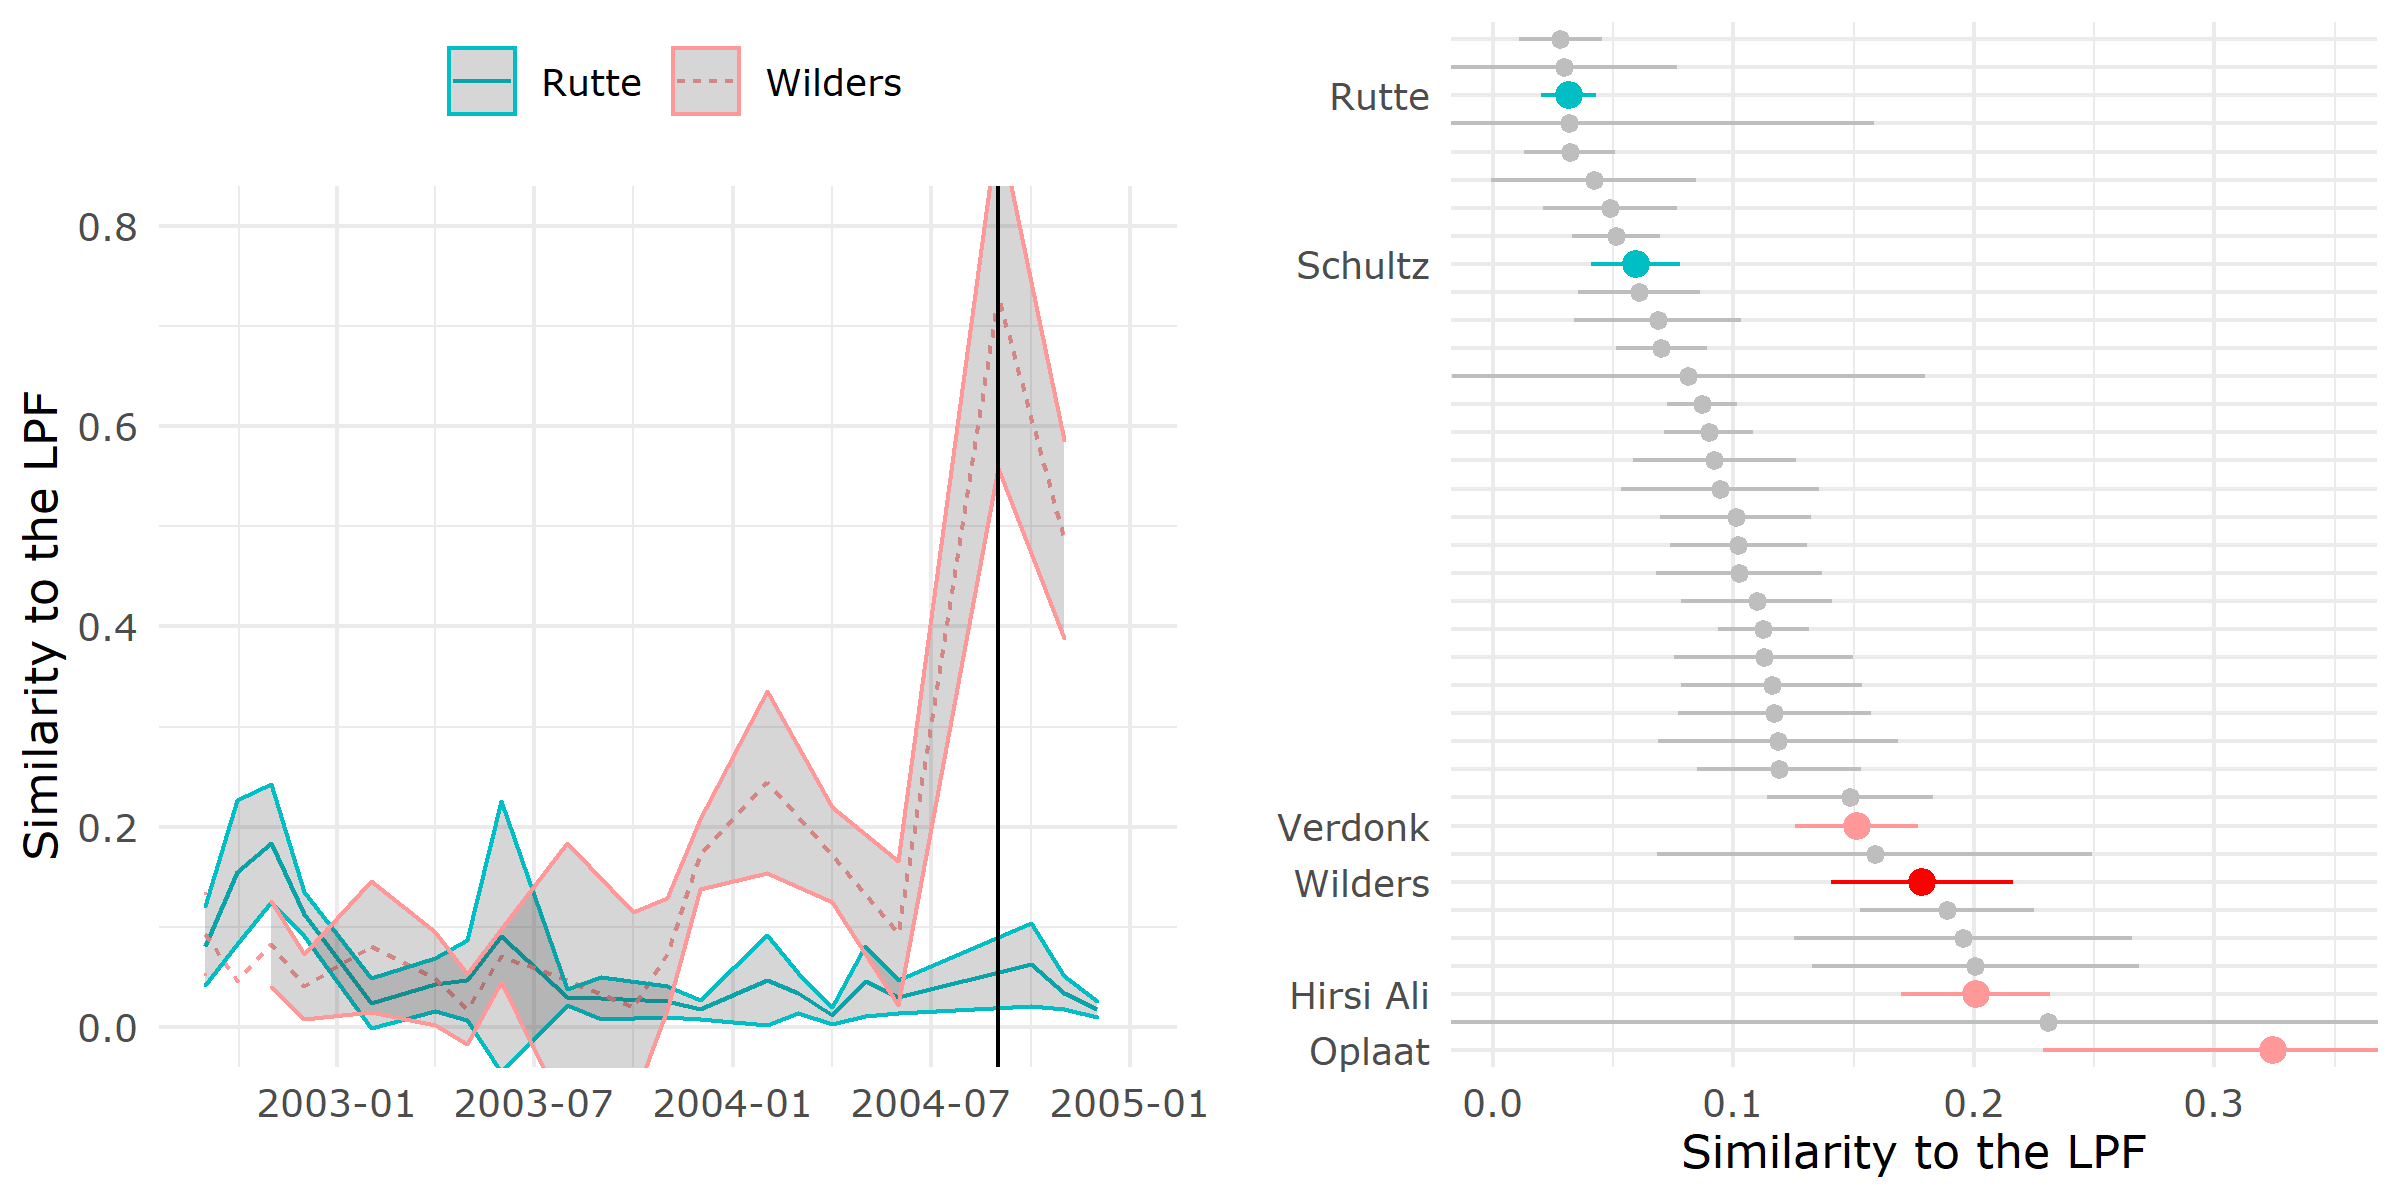
\includegraphics[width = \textwidth]{NL/vis/Wilders_both_r.png}
    \end{figure}
\end{frame}


\section{Comparative performance}

\begin{frame}{Comparable Measures}
\begin{figure}
    \centering
    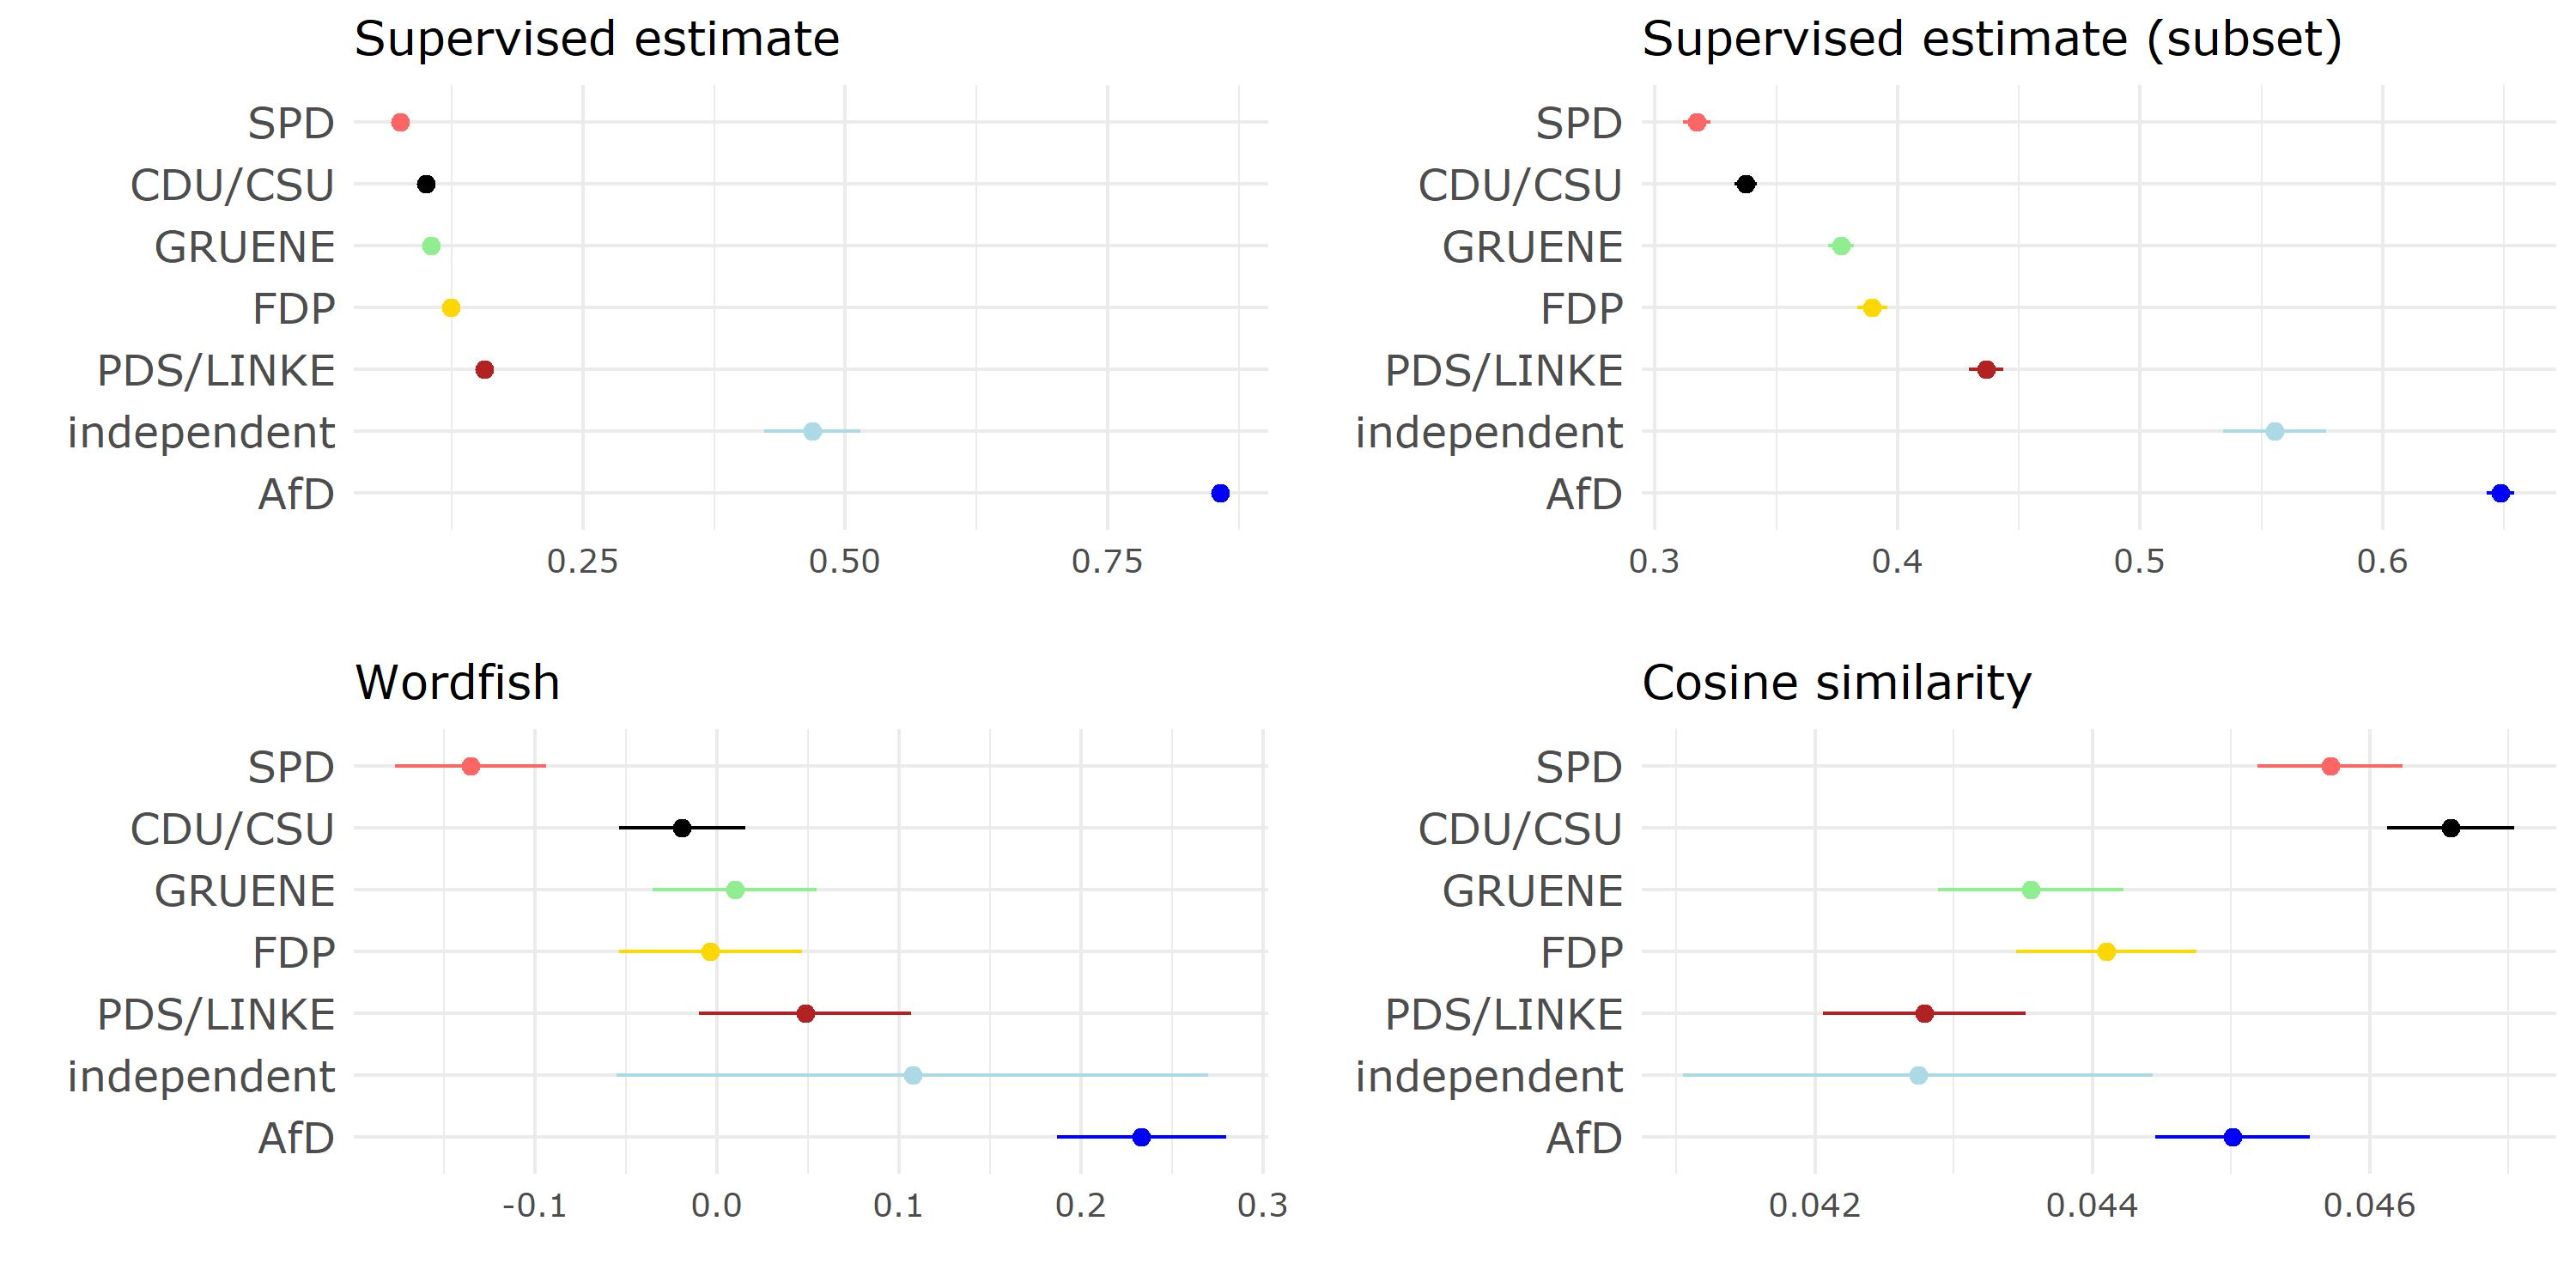
\includegraphics[width = \textwidth]{DE/vis/similarity_pts.jpg}
\end{figure}
\end{frame}


\section{Review}
\begin{frame}{Summary}
\begin{itemize}
    \item SML estimate gives precise measure of rhetorical similarity
    \item the meaning of these differences can be assessed in detail
    \item outperforms other methods like WORDFISH and cosine similarity
\end{itemize}
\end{frame}

\begin{frame}{Reviewer comments}
    \begin{itemize}
        \item Scaling speeches on 'partyness' $\rightarrow$ not a novel method
        \item Doesn't build on \cite{Peterson2018} (scaling, not aggregate accuracy)
        \item Cosine similarity not a measure of similarity (document to corpus)
    \end{itemize}
\end{frame}

\begin{frame}{Possible routes forward}
    Substantive piece
    \begin{itemize}
        \item Testing classical theories of RR accommodation
        \item Improving predictors of coalition formation
        \item Historical: Showing accommodation of NSDAP by conservatives (Levitsky \& Ziblatt)
    \end{itemize}
    
    Methods contribution
    \begin{itemize}
        \item Arguing for extended use of SML for better content validity
        \item Showing a possible application
    \end{itemize}
\end{frame}

\begin{frame}{Thank you!}
    \huge \centering
    Questions?
\end{frame}



\begin{frame}[allowframebreaks]{Resources}
     \printbibliography
\end{frame}

\end{document}
